% Options for packages loaded elsewhere
\PassOptionsToPackage{unicode}{hyperref}
\PassOptionsToPackage{hyphens}{url}
\PassOptionsToPackage{dvipsnames,svgnames,x11names}{xcolor}
%
\documentclass[
]{article}
\usepackage{amsmath,amssymb}
\usepackage{lmodern}
\usepackage{iftex}
\ifPDFTeX
  \usepackage[T1]{fontenc}
  \usepackage[utf8]{inputenc}
  \usepackage{textcomp} % provide euro and other symbols
\else % if luatex or xetex
  \usepackage{unicode-math}
  \defaultfontfeatures{Scale=MatchLowercase}
  \defaultfontfeatures[\rmfamily]{Ligatures=TeX,Scale=1}
\fi
% Use upquote if available, for straight quotes in verbatim environments
\IfFileExists{upquote.sty}{\usepackage{upquote}}{}
\IfFileExists{microtype.sty}{% use microtype if available
  \usepackage[]{microtype}
  \UseMicrotypeSet[protrusion]{basicmath} % disable protrusion for tt fonts
}{}
\makeatletter
\@ifundefined{KOMAClassName}{% if non-KOMA class
  \IfFileExists{parskip.sty}{%
    \usepackage{parskip}
  }{% else
    \setlength{\parindent}{0pt}
    \setlength{\parskip}{6pt plus 2pt minus 1pt}}
}{% if KOMA class
  \KOMAoptions{parskip=half}}
\makeatother
\usepackage{xcolor}
\usepackage[margin=3.5cm]{geometry}
\usepackage{graphicx}
\makeatletter
\def\maxwidth{\ifdim\Gin@nat@width>\linewidth\linewidth\else\Gin@nat@width\fi}
\def\maxheight{\ifdim\Gin@nat@height>\textheight\textheight\else\Gin@nat@height\fi}
\makeatother
% Scale images if necessary, so that they will not overflow the page
% margins by default, and it is still possible to overwrite the defaults
% using explicit options in \includegraphics[width, height, ...]{}
\setkeys{Gin}{width=\maxwidth,height=\maxheight,keepaspectratio}
% Set default figure placement to htbp
\makeatletter
\def\fps@figure{htbp}
\makeatother
\setlength{\emergencystretch}{3em} % prevent overfull lines
\providecommand{\tightlist}{%
  \setlength{\itemsep}{0pt}\setlength{\parskip}{0pt}}
\setcounter{secnumdepth}{-\maxdimen} % remove section numbering
\newlength{\cslhangindent}
\setlength{\cslhangindent}{1.5em}
\newlength{\csllabelwidth}
\setlength{\csllabelwidth}{3em}
\newlength{\cslentryspacingunit} % times entry-spacing
\setlength{\cslentryspacingunit}{\parskip}
\newenvironment{CSLReferences}[2] % #1 hanging-ident, #2 entry spacing
 {% don't indent paragraphs
  \setlength{\parindent}{0pt}
  % turn on hanging indent if param 1 is 1
  \ifodd #1
  \let\oldpar\par
  \def\par{\hangindent=\cslhangindent\oldpar}
  \fi
  % set entry spacing
  \setlength{\parskip}{#2\cslentryspacingunit}
 }%
 {}
\usepackage{calc}
\newcommand{\CSLBlock}[1]{#1\hfill\break}
\newcommand{\CSLLeftMargin}[1]{\parbox[t]{\csllabelwidth}{#1}}
\newcommand{\CSLRightInline}[1]{\parbox[t]{\linewidth - \csllabelwidth}{#1}\break}
\newcommand{\CSLIndent}[1]{\hspace{\cslhangindent}#1}
\ifLuaTeX
  \usepackage{selnolig}  % disable illegal ligatures
\fi
\IfFileExists{bookmark.sty}{\usepackage{bookmark}}{\usepackage{hyperref}}
\IfFileExists{xurl.sty}{\usepackage{xurl}}{} % add URL line breaks if available
\urlstyle{same} % disable monospaced font for URLs
\hypersetup{
  pdftitle={SBMLtoODEjax: efficient simulation and optimization of ODE SBML models in JAX},
  pdfauthor={Mayalen Etcheverry1,2,; Michael Levin3; Clément Moulin-Frier1; Pierre-Yves Oudeyer1},
  colorlinks=true,
  linkcolor={OliveGreen},
  filecolor={Maroon},
  citecolor={OliveGreen},
  urlcolor={OliveGreen},
  pdfcreator={LaTeX via pandoc}}

\title{SBMLtoODEjax: efficient simulation and optimization of ODE SBML
models in JAX}
\author{Mayalen Etcheverry\textsuperscript{1,2,*} \and Michael Levin\textsuperscript{3} \and Clément Moulin-Frier\textsuperscript{1} \and Pierre-Yves Oudeyer\textsuperscript{1}}
\date{}

\begin{document}
\maketitle

\textsuperscript{1} INRIA, University of Bordeaux, Talence 33405,
France\\
\textsuperscript{2} Poietis, Pessac 33600, France\\
\textsuperscript{3} Allen Discovery Center, Tufts University, Medford,
MA, USA

\textsuperscript{*} Correspondence:
\href{mailto:mayalen.etcheverry@inria.fr}{Mayalen Etcheverry
\textless{}mayalen.etcheverry@inria.fr\textgreater{}}

\textbf{Keywords:} SBML, Biological Network Analysis, Python, JAX, high
performance computing, parallel computing

\hypertarget{summary}{%
\section{Summary}\label{summary}}

Developing methods to explore, predict and control the dynamic behavior
of biological systems, from protein pathways to complex cellular
processes, is an essential frontier of research for bioengineering and
biomedicine {[}1{]}. Thus, significant effort has gone in computational
inference and mathematical modeling of biological systems {[}2{]},
{[}3{]}. This effort has resulted in the development of large
collections of publicly-available models, typically stored and exchanged
on online platforms (such as the BioModels Database {[}4{]}, {[}5{]})
using the Systems Biology Markup Language (SBML), a standard format for
representing mathematical models of biological systems {[}6{]}, {[}7{]}.

SBMLtoODEjax is a lightweight library that allows to automatically parse
and convert SBML models into python models written end-to-end in JAX, a
high-performance numerical computing library with automatic
differentiation capabilities {[}8{]}. SBMLtoODEjax is targeted at
researchers that aim to incorporate SBML-specified ordinary differential
equation (ODE) models into their python projects and machine learning
pipelines, in order to perform efficient numerical simulation and
optimization with only a few lines of code. Taking advantage of JAX's
core transformation features, one can easily boost the speed of ODE
models time-course simulations and perform efficient search and
optimization by running simulations in parallel and/or using automatic
differentiation to find derivatives. SBMLtoODEjax extends SBMLtoODEpy, a
python library developed in 2019 for converting SBML files into python
files written in Numpy/Scipy {[}9{]}. The chosen conventions for the
generated variables and modules are slightly different from the standard
SBML conventions (used in the SBMLtoODEpy library) with the aim to
accommodate for more flexible manipulations while preserving JAX-like
functional programming style.

SBMLtoODEjax is available at
\url{https://github.com/flowersteam/sbmltoodejax}.

\hypertarget{statement-of-need}{%
\section{Statement of Need}\label{statement-of-need}}

Despite the wealth of available SBML models, scientists still lack an
in-depth understanding of the range of possible behaviors that these
models can exhibit under different initial data and environmental
stimuli, and lack effective ways to search and optimize those behaviors
via external interventions. Except for a subset of simple networks where
system behavior and response to stimuli can be well understood
analytically (or with exhaustive enumeration methods), onerous sampling
of the parameter space and time-consuming numerical simulations are
often needed which remains a major roadblock for progress in biological
network analysis.

On the other hand, recent progress in machine learning (ML) has led to
the development of novel computational tools that leverage
high-performance computation, parallel execution and differentiable
programming and that promise to accelerate research across multiple
areas of science, including biological network analysis {[}10{]} and
applications in drug discovery and molecular medicine {[}11{]},
{[}12{]}. However, to our knowledge, there is no software tool that
allows seamless integration of existing mathematical models of cellular
molecular pathways (SBML files constructed by biologists) with
ML-supported pipelines and programming frameworks. Whereas there exists
many software tools for manipulation and numerical simulation of SBML
models, they typically rely either on specialized simulation platforms
limiting the flexibility for customization and scripting (such as COPASI
{[}13{]}, {[}14{]}, Virtual Cell {[}15{]}, {[}16{]} and Cell Designer
{[}17{]}, {[}18{]}) or provide scripting interfaces in Python or Matlab
but rely on backend engines that do not support hardware acceleration or
automatic differentiation (like Tellurium {[}19{]}, {[}20{]} and
SBMLtoODEpy {[}9{]} python packages, or the Systems Biology Format
Converter (SBFC) which generates MATLAB and OCTAVE code {[}21{]}).

SBMLtoODEjax seeks to bridge that gap by bringing SBML simulation to the
\href{https://github.com/n2cholas/awesome-jax}{JAX ecosystem}, a
thriving community of JAX libraries that aim to accelerate research in
machine learning and beyond, with diverse applications spanning
molecular dynamics {[}22{]}, protein engineering {[}23{]}, quantum
physics {[}24{]}, cosmology {[}25{]}, ocean modeling {[}26{]},
photovoltaic research {[}27{]}, acoustic simulations {[}28{]} and fluid
dynamics {[}29{]}. SBMLtoODEjax aims to integrate this ecosystem and
provide tools to accelerate research in biological network analysis.

\hypertarget{why-use-sbmltoodejax}{%
\section{Why use SBMLtoODEjax?}\label{why-use-sbmltoodejax}}

\textbf{\emph{Simplicity and extensibility}} SBMLtoODEjax retains the
simplicity of the SBMLtoODEPy library to facilitate incorporation and
refactoring of the ODE models into one's own python projects. As shown
in \autoref{fig:fig1}, with only a few lines of python code one can load
and simulate existing SBML files.

\begin{figure}
\centering
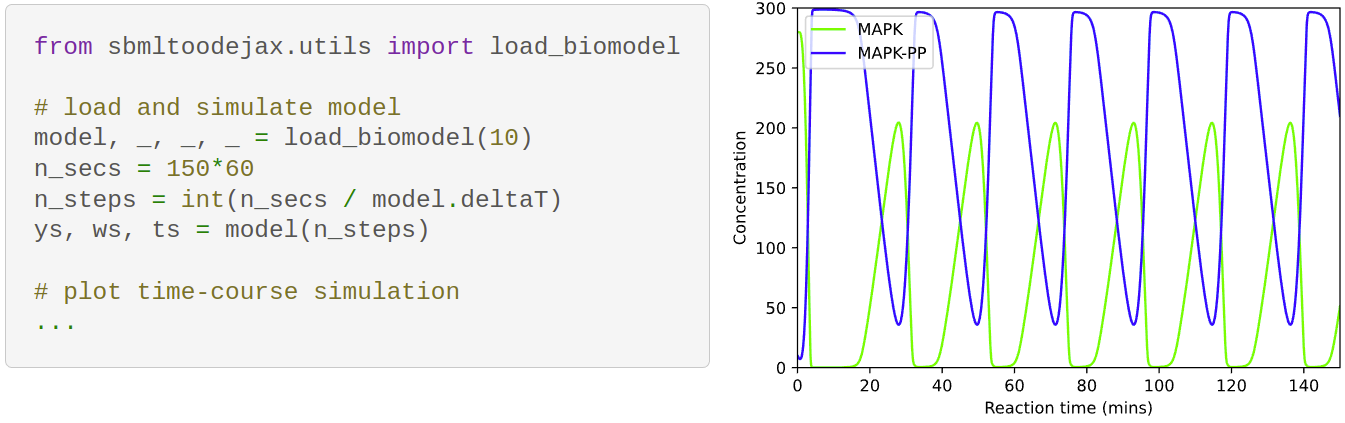
\includegraphics[width=0.8\textwidth,height=\textheight]{fig1.png}
\caption{Example code (left) and output snapshot (right) reproducing
\href{https://www.ebi.ac.uk/biomodels/BIOMD0000000010\#Curation}{original
simulation results} of Kholodenko 2000's paper {[}30{]} hosted on
BioModels website. \label{fig:fig1}}
\end{figure}

\textbf{\emph{JAX-friendly}} The generated python models are tailored to
take advantage of JAX main features. Model rollouts use \texttt{jit}
transformation and \texttt{scan} primitive to reduce compilation and
execution time of the recursive ODE integration steps, which is
particularly useful when running large numbers of steps (long reaction
times). Models also inherit from the Equinox module abstraction {[}31{]}
and are registered as PyTree containers, which facilitates the
application of JAX core transformations to any SBMLtoODEjax object.

\textbf{\emph{Efficiency simulation and optimization}} The application
of JAX core transformations, such as just-in-time compilation
(\texttt{jit}), automatic vectorization (\texttt{vmap}) and automatic
differentiation (\texttt{grad}), to the generated models make it very
easy (and seamless) to efficiently run simulations in parallel. For
instance, as shown in \autoref{fig:fig2}, with only a few lines of
python code one can vectorize calls to model rollout and perform batched
computations efficiently, which is particularly useful when considering
large batch sizes.

\begin{figure}
\centering
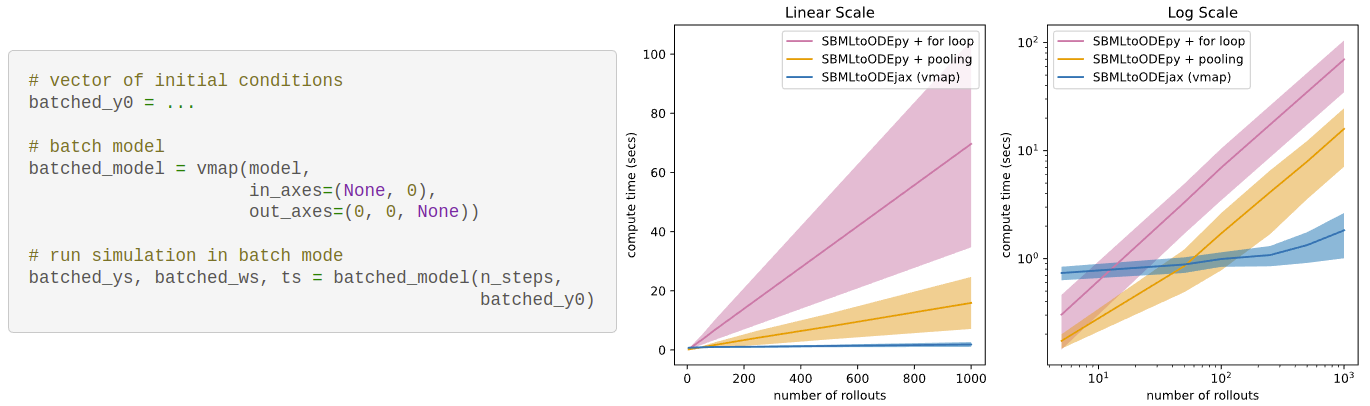
\includegraphics[width=1\textwidth,height=\textheight]{fig2.png}
\caption{(left) Example code to vectorize calls to model rollout (right)
Results of a (rudimentary) benchmark comparing the average simulation
time of models implemented with SBMLtoODEpy versus SBMLtoODEjax (for
different number of rollouts i.e.~batch size). For additional details on
the comparison, please refer to our
\href{https://developmentalsystems.org/sbmltoodejax/tutorials/benchmark.html}{Benchmarking}
notebook. \label{fig:fig2}}
\end{figure}

As shown in \autoref{fig:fig3}, SBMLtoODEjax models can also be
integrated within Optax pipelines, a gradient processing and
optimization library for JAX {[}32{]}, allowing to optimize model
parameters and/or external interventions with stochastic gradient
descent.

\begin{figure}
\centering
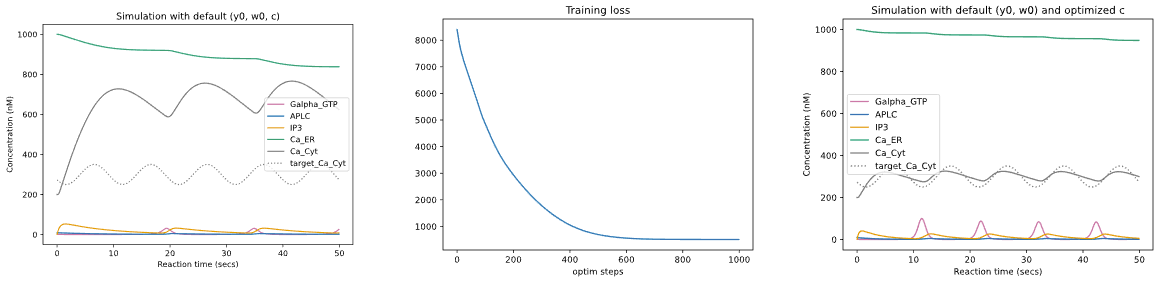
\includegraphics[width=1\textwidth,height=\textheight]{fig3.png}
\caption{(left) Default simulation results of
\href{https://www.ebi.ac.uk/biomodels/BIOMD0000000145}{biomodel \#145}
which models ATP-induced intracellular calcium oscillations, and
(arbitrary) target sine-wave pattern for Ca\_Cyt concentration. (middle)
Training loss obtained when running the Optax optimization loop, with
Adam optimizer, over the model kinematic parameters \(c\). (right)
Simulation results obtained after optimization. The full example is
available at our
\href{https://developmentalsystems.org/sbmltoodejax/tutorials/gradient_descent.html}{Gradient
Descent} tutorial. \label{fig:fig3}}
\end{figure}

Altogether, the parallel execution capabilities and the
differentiability of the generated models opens interesting
possibilities to design and optimize intervention strategies.

\textbf{\emph{Current limitations}} SBMLtoODEjax is still in its early
phase and does not yet handle all possible cases of SBML files, but we
welcome contributions and aim to handle more cases in future releases.
Similarly, SBMLtoODEjax only integrates one ODE solver for now
(\texttt{jax.experimental.odeint}), but could benefit from more
{[}33{]}. Finally, whereas SBMLtoODEjax is to our knowledge the first
software tool enabling gradient backpropagation through the SBML model
rollout, applying it in practice can be hard and other optimization
methods, such as evolutionary strategies, might be more adapted.

\textbf{\emph{Documentation}} Please refer to
\url{https://developmentalsystems.org/sbmltoodejax/} for additional
details on SBMLtoODEjax's main
\href{https://developmentalsystems.org/sbmltoodejax/design_principles.html}{design
principles},
\href{https://developmentalsystems.org/sbmltoodejax/why_use.html}{advantages
and limitations}, and API docs as well as for various hands-on tutorials
for
\href{https://developmentalsystems.org/sbmltoodejax/tutorials/biomodels_curation.html}{loading
and simulating biomodels},
\href{https://developmentalsystems.org/sbmltoodejax/tutorials/parallel_execution.html}{parallel
execution} and
\href{https://developmentalsystems.org/sbmltoodejax/tutorials/gradient_descent.html}{gradient
descent}.

\hypertarget{software-requirements}{%
\section{Software requirements}\label{software-requirements}}

SBMLtoODEjax is developed under the MIT license and available on
\texttt{PyPI} via \texttt{pip\ install\ sbmltoodejax}. It is written on
top of SBMLtoODEpy {[}9{]}, JAX (cpu) {[}8{]} and Equinox {[}31{]},
which are the main requirements.

\hypertarget{acknowledgements}{%
\section{Acknowledgements}\label{acknowledgements}}

SBMLtoODEjax builds on SBMLtoODEpy's parsing and conversion of SBML
files {[}9{]}, JAX's composable transformations {[}8{]}, Equinox's
module abstraction {[}31{]} and BasiCO's access to the BioModels REST
api {[}14{]}.

This work has been funded by the biotechnology company Poietis and the
French National Association of Research and Technology (ANRT), as well
as by the French National Research Agency (ANR, project DeepCuriosity).
It also benefited from two mobility research scholarships given by the
French Academy (Jean Walter Zellidja scholarship) and the University of
Bordeaux (UBGRS-Mob scholarship). Finally, this work benefited from the
use of the Jean Zay supercomputer associated with the Genci grant
A0091011996.

\hypertarget{references}{%
\section*{References}\label{references}}
\addcontentsline{toc}{section}{References}

\hypertarget{refs}{}
\begin{CSLReferences}{0}{0}
\leavevmode\vadjust pre{\hypertarget{ref-kitanoSystemsBiologyBrief2002}{}}%
\CSLLeftMargin{{[}1{]} }%
\CSLRightInline{H. Kitano, {``Systems {Biology}: {A Brief Overview},''}
\emph{Science}, vol. 295, no. 5560, pp. 1662--1664, Mar. 2002, doi:
\href{https://doi.org/10.1126/science.1069492}{10.1126/science.1069492}.}

\leavevmode\vadjust pre{\hypertarget{ref-dejongModelingSimulationGenetic2002}{}}%
\CSLLeftMargin{{[}2{]} }%
\CSLRightInline{H. de Jong, {``Modeling and {Simulation} of {Genetic
Regulatory Systems}: {A Literature Review},''} \emph{Journal of
Computational Biology}, vol. 9, no. 1, pp. 67--103, Jan. 2002, doi:
\href{https://doi.org/10.1089/10665270252833208}{10.1089/10665270252833208}.}

\leavevmode\vadjust pre{\hypertarget{ref-delgadoComputationalMethodsGene2019}{}}%
\CSLLeftMargin{{[}3{]} }%
\CSLRightInline{F. M. Delgado and F. Gómez-Vela, {``Computational
methods for {Gene Regulatory Networks} reconstruction and analysis: {A}
review,''} \emph{Artificial Intelligence in Medicine}, vol. 95, pp.
133--145, Apr. 2019, doi:
\href{https://doi.org/10.1016/j.artmed.2018.10.006}{10.1016/j.artmed.2018.10.006}.}

\leavevmode\vadjust pre{\hypertarget{ref-glontBioModelsExpandingHorizons2018}{}}%
\CSLLeftMargin{{[}4{]} }%
\CSLRightInline{M. Glont \emph{et al.}, {``{BioModels}: Expanding
horizons to include more modelling approaches and formats,''}
\emph{Nucleic Acids Research}, vol. 46, no. D1, pp. D1248--D1253, Jan.
2018, doi:
\href{https://doi.org/10.1093/nar/gkx1023}{10.1093/nar/gkx1023}.}

\leavevmode\vadjust pre{\hypertarget{ref-malik-sheriffBioModels15Years2020a}{}}%
\CSLLeftMargin{{[}5{]} }%
\CSLRightInline{R. S. Malik-Sheriff \emph{et al.},
{``{BioModels}\textemdash 15 years of sharing computational models in
life science,''} \emph{Nucleic Acids Research}, vol. 48, no. D1, pp.
D407--D415, Jan. 2020, doi:
\href{https://doi.org/10.1093/nar/gkz1055}{10.1093/nar/gkz1055}.}

\leavevmode\vadjust pre{\hypertarget{ref-huckaSystemsBiologyMarkup2003}{}}%
\CSLLeftMargin{{[}6{]} }%
\CSLRightInline{M. Hucka \emph{et al.}, {``The systems biology markup
language ({SBML}): A medium for representation and exchange of
biochemical network models,''} \emph{Bioinformatics}, vol. 19, no. 4,
pp. 524--531, Mar. 2003, doi:
\href{https://doi.org/10.1093/bioinformatics/btg015}{10.1093/bioinformatics/btg015}.}

\leavevmode\vadjust pre{\hypertarget{ref-huckaSystemsBiologyMarkup2019}{}}%
\CSLLeftMargin{{[}7{]} }%
\CSLRightInline{M. Hucka \emph{et al.}, {``The {Systems Biology Markup
Language} ({SBML}): {Language Specification} for {Level} 3 {Version} 2
{Core Release} 2,''} \emph{Journal of Integrative Bioinformatics}, vol.
16, no. 2, p. 20190021, Jun. 2019, doi:
\href{https://doi.org/10.1515/jib-2019-0021}{10.1515/jib-2019-0021}.}

\leavevmode\vadjust pre{\hypertarget{ref-jax2018github}{}}%
\CSLLeftMargin{{[}8{]} }%
\CSLRightInline{J. Bradbury \emph{et al.}, {``{JAX}: Composable
transformations of {Python}+{NumPy} programs.''} 2018.}

\leavevmode\vadjust pre{\hypertarget{ref-ruggieroSBMLtoODEpySoftwareProgram2019}{}}%
\CSLLeftMargin{{[}9{]} }%
\CSLRightInline{S. M. Ruggiero and A. N. F. Versypt, {``{SBMLtoODEpy}:
{A} software program for converting {SBML} models into {ODE} models in
{Python},''} \emph{Journal of Open Source Software}, vol. 5, no. 53, p.
1643, Sep. 2019, doi:
\href{https://doi.org/10.21105/joss.01643}{10.21105/joss.01643}.}

\leavevmode\vadjust pre{\hypertarget{ref-muzioBiologicalNetworkAnalysis2021}{}}%
\CSLLeftMargin{{[}10{]} }%
\CSLRightInline{G. Muzio, L. O'Bray, and K. Borgwardt, {``Biological
network analysis with deep learning,''} \emph{Briefings in
Bioinformatics}, vol. 22, no. 2, pp. 1515--1530, Mar. 2021, doi:
\href{https://doi.org/10.1093/bib/bbaa257}{10.1093/bib/bbaa257}.}

\leavevmode\vadjust pre{\hypertarget{ref-camachoNextGenerationMachineLearning2018a}{}}%
\CSLLeftMargin{{[}11{]} }%
\CSLRightInline{D. M. Camacho, K. M. Collins, R. K. Powers, J. C.
Costello, and J. J. Collins, {``Next-{Generation Machine Learning} for
{Biological Networks},''} \emph{Cell}, vol. 173, no. 7, pp. 1581--1592,
Jun. 2018, doi:
\href{https://doi.org/10.1016/j.cell.2018.05.015}{10.1016/j.cell.2018.05.015}.}

\leavevmode\vadjust pre{\hypertarget{ref-alquraishiDifferentiableBiologyUsing2021}{}}%
\CSLLeftMargin{{[}12{]} }%
\CSLRightInline{M. AlQuraishi and P. K. Sorger, {``Differentiable
biology: Using deep learning for biophysics-based and data-driven
modeling of molecular mechanisms,''} \emph{Nature Methods}, vol. 18, no.
10, pp. 1169--1180, Oct. 2021, doi:
\href{https://doi.org/10.1038/s41592-021-01283-4}{10.1038/s41592-021-01283-4}.}

\leavevmode\vadjust pre{\hypertarget{ref-hoopsCOPASICOmplexPAthway2006}{}}%
\CSLLeftMargin{{[}13{]} }%
\CSLRightInline{S. Hoops \emph{et al.}, {``{COPASI}\textemdash a
{COmplex PAthway SImulator},''} \emph{Bioinformatics}, vol. 22, no. 24,
pp. 3067--3074, Dec. 2006, doi:
\href{https://doi.org/10.1093/bioinformatics/btl485}{10.1093/bioinformatics/btl485}.}

\leavevmode\vadjust pre{\hypertarget{ref-Bergmann_copasi_basico_Release_0_48_2023}{}}%
\CSLLeftMargin{{[}14{]} }%
\CSLRightInline{F. T. Bergmann, {``Copasi/basico: {Release} 0.48.''}
Mar. 2023.}

\leavevmode\vadjust pre{\hypertarget{ref-loewVirtualCellSoftware2001}{}}%
\CSLLeftMargin{{[}15{]} }%
\CSLRightInline{L. M. Loew and J. C. Schaff, {``The {Virtual Cell}: A
software environment for computational cell biology,''} \emph{Trends in
Biotechnology}, vol. 19, no. 10, pp. 401--406, Oct. 2001, doi:
\href{https://doi.org/10.1016/S0167-7799(01)01740-1}{10.1016/S0167-7799(01)01740-1}.}

\leavevmode\vadjust pre{\hypertarget{ref-slepchenkoQuantitativeCellBiology2003a}{}}%
\CSLLeftMargin{{[}16{]} }%
\CSLRightInline{B. M. Slepchenko, J. C. Schaff, I. Macara, and L. M.
Loew, {``Quantitative cell biology with the {Virtual Cell},''}
\emph{Trends in Cell Biology}, vol. 13, no. 11, pp. 570--576, Nov. 2003,
doi:
\href{https://doi.org/10.1016/j.tcb.2003.09.002}{10.1016/j.tcb.2003.09.002}.}

\leavevmode\vadjust pre{\hypertarget{ref-funahashiCellDesignerProcessDiagram2003}{}}%
\CSLLeftMargin{{[}17{]} }%
\CSLRightInline{A. Funahashi, M. Morohashi, H. Kitano, and N. Tanimura,
{``{CellDesigner}: A process diagram editor for gene-regulatory and
biochemical networks,''} \emph{BIOSILICO}, vol. 1, no. 5, pp. 159--162,
Nov. 2003, doi:
\href{https://doi.org/10.1016/S1478-5382(03)02370-9}{10.1016/S1478-5382(03)02370-9}.}

\leavevmode\vadjust pre{\hypertarget{ref-funahashiCellDesignerVersatileModeling2008}{}}%
\CSLLeftMargin{{[}18{]} }%
\CSLRightInline{A. Funahashi, Y. Matsuoka, A. Jouraku, M. Morohashi, N.
Kikuchi, and H. Kitano, {``{CellDesigner} 3.5: {A Versatile Modeling
Tool} for {Biochemical Networks},''} \emph{Proceedings of the IEEE},
vol. 96, no. 8, pp. 1254--1265, Aug. 2008, doi:
\href{https://doi.org/10.1109/JPROC.2008.925458}{10.1109/JPROC.2008.925458}.}

\leavevmode\vadjust pre{\hypertarget{ref-choiTelluriumExtensiblePythonbased2018}{}}%
\CSLLeftMargin{{[}19{]} }%
\CSLRightInline{K. Choi \emph{et al.}, {``Tellurium: {An} extensible
python-based modeling environment for systems and synthetic biology,''}
\emph{Biosystems}, vol. 171, pp. 74--79, Sep. 2018, doi:
\href{https://doi.org/10.1016/j.biosystems.2018.07.006}{10.1016/j.biosystems.2018.07.006}.}

\leavevmode\vadjust pre{\hypertarget{ref-medleyTelluriumNotebooksEnvironment2018}{}}%
\CSLLeftMargin{{[}20{]} }%
\CSLRightInline{J. K. Medley \emph{et al.}, {``Tellurium
notebooks\textemdash{{An}} environment for reproducible dynamical
modeling in systems biology,''} \emph{PLOS Computational Biology}, vol.
14, no. 6, p. e1006220, Jun. 2018, doi:
\href{https://doi.org/10.1371/journal.pcbi.1006220}{10.1371/journal.pcbi.1006220}.}

\leavevmode\vadjust pre{\hypertarget{ref-rodriguezSystemsBiologyFormat2016}{}}%
\CSLLeftMargin{{[}21{]} }%
\CSLRightInline{N. Rodriguez \emph{et al.}, {``The systems biology
format converter,''} \emph{BMC Bioinformatics}, vol. 17, no. 1, p. 154,
Apr. 2016, doi:
\href{https://doi.org/10.1186/s12859-016-1000-2}{10.1186/s12859-016-1000-2}.}

\leavevmode\vadjust pre{\hypertarget{ref-schoenholzJAXFrameworkDifferentiable2020}{}}%
\CSLLeftMargin{{[}22{]} }%
\CSLRightInline{S. S. Schoenholz and E. D. Cubuk, {``{JAX}, {M}.{D}.: {A
Framework} for {Differentiable Physics}.''} {arXiv}, Dec. 2020.
Accessed: Jun. 02, 2023. {[}Online{]}. Available:
\url{https://arxiv.org/abs/1912.04232}}

\leavevmode\vadjust pre{\hypertarget{ref-maReimplementingUnirepJAX2020}{}}%
\CSLLeftMargin{{[}23{]} }%
\CSLRightInline{E. J. Ma and A. Kummer, {``Reimplementing {Unirep} in
{JAX}.''} {bioRxiv}, p. 2020.05.11.088344, May 2020. doi:
\href{https://doi.org/10.1101/2020.05.11.088344}{10.1101/2020.05.11.088344}.}

\leavevmode\vadjust pre{\hypertarget{ref-carleoNetKetMachineLearning2019}{}}%
\CSLLeftMargin{{[}24{]} }%
\CSLRightInline{G. Carleo \emph{et al.}, {``{NetKet}: {A} machine
learning toolkit for many-body quantum systems,''} \emph{SoftwareX},
vol. 10, p. 100311, Jul. 2019, doi:
\href{https://doi.org/10.1016/j.softx.2019.100311}{10.1016/j.softx.2019.100311}.}

\leavevmode\vadjust pre{\hypertarget{ref-campagneJAXCOSMOEndtoEndDifferentiable2023}{}}%
\CSLLeftMargin{{[}25{]} }%
\CSLRightInline{J.-E. Campagne \emph{et al.}, {``{JAX-COSMO}: {An
End-to-End Differentiable} and {GPU Accelerated Cosmology Library},''}
\emph{The Open Journal of Astrophysics}, vol. 6, p.
10.21105/astro.2302.05163, Apr. 2023, doi:
\href{https://doi.org/10.21105/astro.2302.05163}{10.21105/astro.2302.05163}.}

\leavevmode\vadjust pre{\hypertarget{ref-hafnerFastCheapTurbulent2021}{}}%
\CSLLeftMargin{{[}26{]} }%
\CSLRightInline{D. Häfner, R. Nuterman, and M. Jochum, {``Fast, {Cheap},
and
{Turbulent}\textemdash{{Global Ocean Modeling With GPU Acceleration}} in
{Python},''} \emph{Journal of Advances in Modeling Earth Systems}, vol.
13, no. 12, p. e2021MS002717, 2021, doi:
\href{https://doi.org/10.1029/2021MS002717}{10.1029/2021MS002717}.}

\leavevmode\vadjust pre{\hypertarget{ref-mannPVEndtoendDifferentiable2022}{}}%
\CSLLeftMargin{{[}27{]} }%
\CSLRightInline{S. Mann, E. Fadel, S. S. Schoenholz, E. D. Cubuk, S. G.
Johnson, and G. Romano, {``{\(\partial\)}{PV}: {An} end-to-end
differentiable solar-cell simulator,''} \emph{Computer Physics
Communications}, vol. 272, p. 108232, Mar. 2022, doi:
\href{https://doi.org/10.1016/j.cpc.2021.108232}{10.1016/j.cpc.2021.108232}.}

\leavevmode\vadjust pre{\hypertarget{ref-stanziolaJWaveOpensourceDifferentiable2023}{}}%
\CSLLeftMargin{{[}28{]} }%
\CSLRightInline{A. Stanziola, S. R. Arridge, B. T. Cox, and B. E.
Treeby, {``J-{Wave}: {An} open-source differentiable wave simulator,''}
\emph{SoftwareX}, vol. 22, p. 101338, May 2023, doi:
\href{https://doi.org/10.1016/j.softx.2023.101338}{10.1016/j.softx.2023.101338}.}

\leavevmode\vadjust pre{\hypertarget{ref-bezginJAXFluidsFullydifferentiableHighorder2023}{}}%
\CSLLeftMargin{{[}29{]} }%
\CSLRightInline{D. A. Bezgin, A. B. Buhendwa, and N. A. Adams,
{``{JAX-Fluids}: {A} fully-differentiable high-order computational fluid
dynamics solver for compressible two-phase flows,''} \emph{Computer
Physics Communications}, vol. 282, p. 108527, Jan. 2023, doi:
\href{https://doi.org/10.1016/j.cpc.2022.108527}{10.1016/j.cpc.2022.108527}.}

\leavevmode\vadjust pre{\hypertarget{ref-kholodenkoNegativeFeedbackUltrasensitivity2000}{}}%
\CSLLeftMargin{{[}30{]} }%
\CSLRightInline{B. N. Kholodenko, {``Negative feedback and
ultrasensitivity can bring about oscillations in the mitogen-activated
protein kinase cascades,''} \emph{European Journal of Biochemistry},
vol. 267, no. 6, pp. 1583--1588, Mar. 2000, doi:
\href{https://doi.org/10.1046/j.1432-1327.2000.01197.x}{10.1046/j.1432-1327.2000.01197.x}.}

\leavevmode\vadjust pre{\hypertarget{ref-kidger2021equinox}{}}%
\CSLLeftMargin{{[}31{]} }%
\CSLRightInline{P. Kidger and C. Garcia, {``Equinox: Neural networks in
{JAX} via callable {PyTrees} and filtered transformations,''}
\emph{Differentiable Programming workshop at Neural Information
Processing Systems 2021}, 2021.}

\leavevmode\vadjust pre{\hypertarget{ref-deepmind2020jax}{}}%
\CSLLeftMargin{{[}32{]} }%
\CSLRightInline{I. Babuschkin \emph{et al.}, {``The {DeepMind JAX
Ecosystem}.''} 2020.}

\leavevmode\vadjust pre{\hypertarget{ref-stadterBenchmarkingNumericalIntegration2021a}{}}%
\CSLLeftMargin{{[}33{]} }%
\CSLRightInline{P. Städter, Y. Schälte, L. Schmiester, J. Hasenauer, and
P. L. Stapor, {``Benchmarking of numerical integration methods for {ODE}
models of biological systems,''} \emph{Scientific Reports}, vol. 11, no.
1, p. 2696, Jan. 2021, doi:
\href{https://doi.org/10.1038/s41598-021-82196-2}{10.1038/s41598-021-82196-2}.}

\end{CSLReferences}

\end{document}
